\subsection{Raspberry Pi}\label{ss:Raspberry}

Die in Großbritannien angesiedelte Wohltätigkeitsorganisation "Raspberry Pi Foundation" hat es sich zur Aufgabe gemacht, Einplatinencomputer für Menschen zu entwickeln, die Hardware- oder Programmierkenntnisse erwerben wollen. Um auch für Jugendliche und Studenten ansprechend zu sein, wurde ein besonders geringer Verkaufspreis angestrebt. Die verschiedenen Modelle des Raspberry Pis kosten zwischen 20 und 35 US-\$ und sind somit sehr günstig.\\

Der Name setzt entstand durch die aus der Kombination zweier Gedanken. Viele Computer wurden nach Früchten benannt (z.B. Apple), aus diesem Grund entschieden sich die Gründer für Raspberry. Der Namenszusatz Pi entstand aus dem Ursprünglichen plan, die Raspberry Pi Einplatinencomputer mit einem Phyton Interpreter auszuliefern, daher das die Abkürzung PI. Als Ergebnis eines öffentlich ausgeschrieben Wettbewerbs wurde eine silisierte Himbeere als Logo für die Wohltätigkeitsorganisation gewählt.

\begin{figure}[H] 
	\centering
	
\includegraphics[scale=0.15]{Bilder/raspberrylogo}
	\caption{Das Logo der Raspberry Pi Foundation\cite{i:raspberrylogo}}
	\label{f:raspberrylogo}
\end{figure}

Insgesamt bietet die Raspberry Pi Foundation sechs Modelle des Computers an. Eine sehr grundlegende ausführung, das Compute Module, dass nur in Stückzahlen über 100 verkauft wird, sowie die günstigen Modelle A und A+, die mit 25 und 20 US-\$ am unteren Preisende liegen. Die Modelle B, B+, sowie das überarbeitete Modell Generation 2 B sind am oberne Preisende, mit jeweils 35 US-\$ angesiedelt. \\

\begin{figure}[H] 
	\centering
	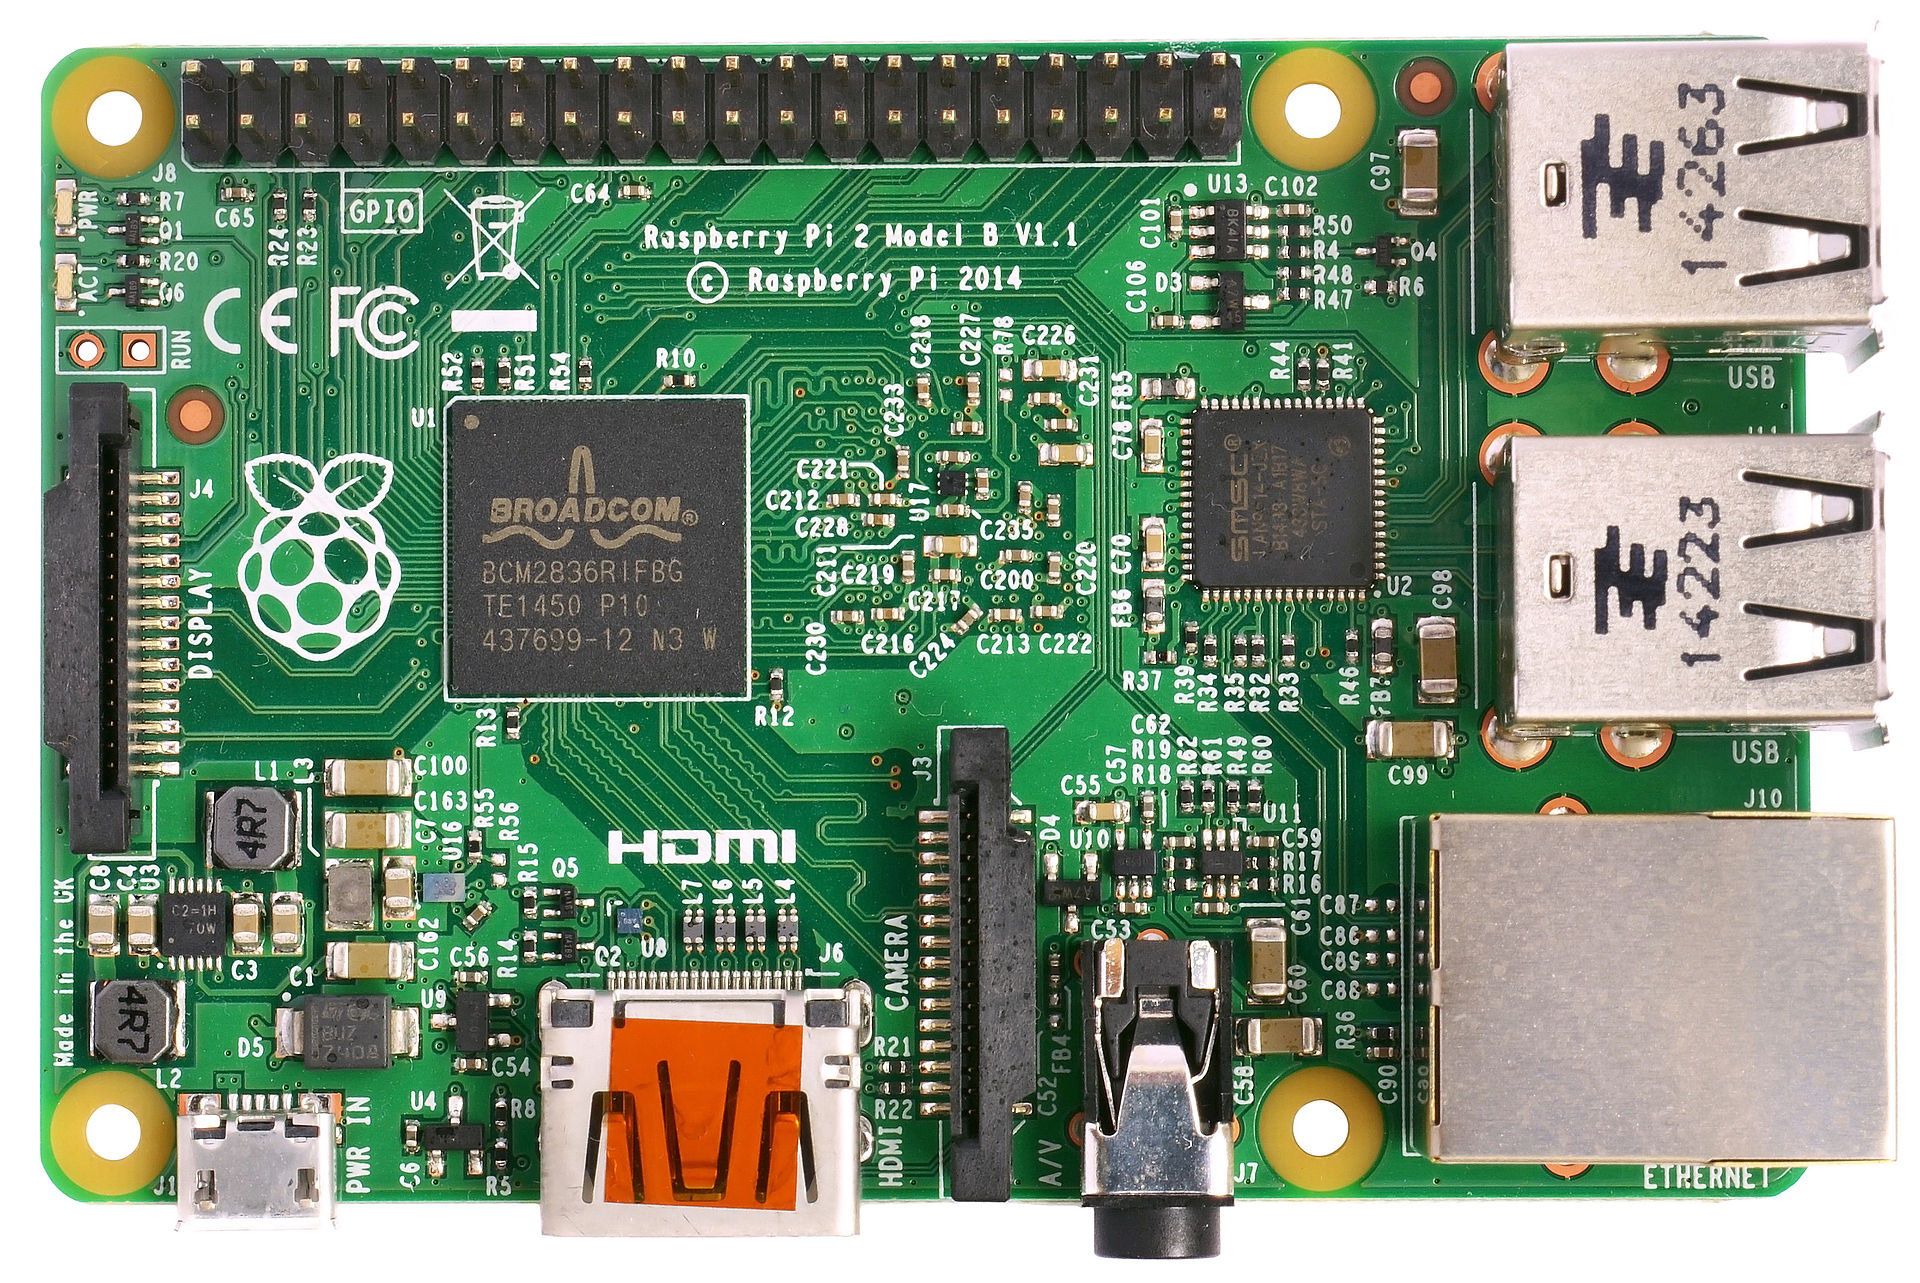
\includegraphics[scale=0.5]{Bilder/raspberry2top}
	\caption{Die Oberseite des Raspberry Generation 2 B-Modells\cite{i:raspberry2top}}
	\label{f:raspberry2top}
\end{figure}

Mit dem Anfang 2015 vorgestellten Generation 2 B - Modell wurde ein Performancesprung realisiert. 
Mit dem System-on-a-Chip Broadcom BCM2836, das sowohl CPU als auch GPU des Einplatinencomputers darstellt sind auf vier Kernen berechnungen mit bis zu 900 \ac{Mhz} möglich. Dies wird mit 1 Gigabyte Arbeitsspeicher zu einem, für den geringen Preis, leistungsstarken System kombiniert.
Die Hardwarekomponenten des Generation 2 B -Modells sind so leistungsstark, dass das Ausführen von Windows 10 möglich ist.\\

Auch in Sachen I/O-Anschlüsse ist der Raspberry Pi gut ausgerüstet. Er stellt insgesamt 17 Pins bereit, die sowohl als Input, sowie Output genutzt werden können. Zusätzlich verfügt der Raspberry Pi über 4 \ac{USB}-Ports, einen HDMI-Anschluss und einen MicroSD-Karten Slot. Dieser wird als Speicher für das Betriebssystem und alle selbstentwickelten Programme verwendet.\\
Um den Raspberry Pi mit Netzwerken zu verbinden besitzt der Raspberry ein 100Mbit Ethernet Port. Zusätzlich sind viele Treiber vorinstalliert, die die Verwendung von USB-WLAN-Adaptern ermöglichen. 

Über Micro-\ac{USB} wird die Platine mit 5V versorgt, die sich mit der Stromstärke von bis zu 800mA auf 4 Watt aufsummieren. \\

Um Hardwareerweiterungen zu ermöglichen bietet der Raspberry Pi einen seriellen Anschluss. Eine beliebte Erweiterung ist das Camera Module, das wie der Name bereits sagt, eine Kamera mit sich bringt. Diese besitzt eine Auflösung von fünf Megapixel und ist besonders für Überwachungsszenarien beliebt. Um auch Nachts oder in schwach belichteten Umgebungen Aufnahmen tätigen zu können, ist das Camera Modul unter dem Namen NoIR ohne Infrarotfilter erhältlich. Dies ermöglicht in Kombination mit Infrarotlicht aufnahmen in Dunkelheit.

\begin{figure}[H] 
	\centering
	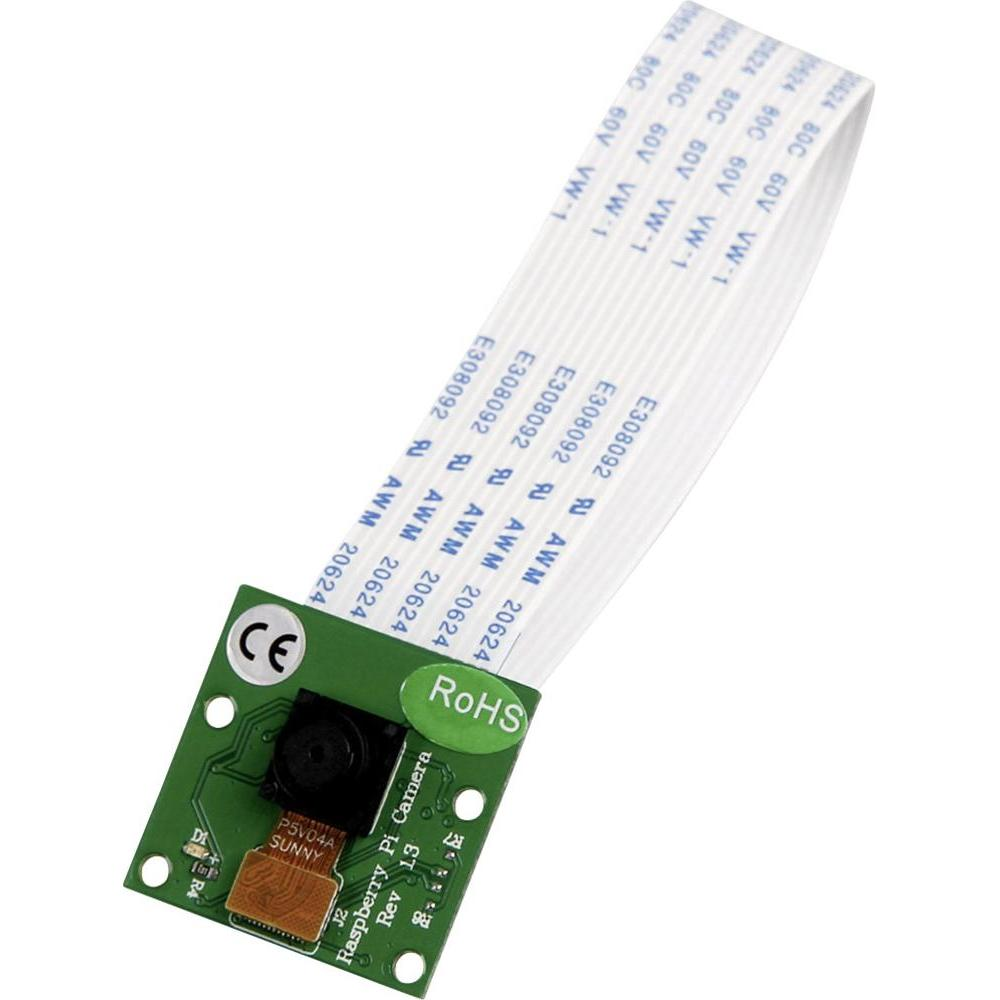
\includegraphics[scale=0.2]{Bilder/cameramodul}
	\caption{Das Camera Modul für den Raspberry Pi\cite{i:camera}}
	\label{f:camera}
\end{figure}

Der Raspberry Pi ist mit seinen 85 x 56mm so groß wie eine Kreditkarte. Zusätzlich zum platzsparenden Format ist der Einplatinencomputer mit 45 gramm ein Leichtgewicht.